
\section{Test} % (fold)
\label{sec:test}
    
    I test sono stati condotti utilizzando le seguenti meta--euristiche.
    \begin{itemize}
        \item[--] \emph{simulated annealing} con mossa 3--modale SEO (\emph{Singleton} move, \emph{Even Chessboard} Move, \emph{Odd Chessboard} Move);
        \item[--] \emph{simulated annealing} con mossa 3--modale STL (\emph{Singleton} move, \emph{Three-Tile Streak} Move, \emph{L} Move);
        \item[--] \emph{steepest descent} con mossa 5--modale (\emph{Singleton} move, \emph{Even Chessboard} Move, \emph{Odd Chessboard} Move, \emph{Three-Tile Streak} Move, \emph{L} Move );
    \end{itemize}

    Sulla base delle funzioni offerte da easylocal++, la strategia \emph{steepest descent} con la mossa 5--modale chiama la BestMove usando l'enumerazione completa per le cinque mosse componenti. Per questo motivo, si è scelto di implementare la \emph{steepest descent} esternamente al framework, usando il \emph{tester} di easylocal++. In questo senso, si chiama il tester da terminale e si redirige in input a tale processo un file con i comandi per il tester, in modo che questi chiamino la BestMove delle cinque mosse. Un esempio è il seguente:

    \begin{center}
	\texttt{./Eternity2 --main::instance ../eternity2-data/pieces\_set\_2/e2pieces.txt --main::seed 987 $<$ ../eternity2-data/ourInput/input\_e2.txt $\mid$ tail -n 50}
	\end{center}

	I risultati verranno visualizzati tramite il seguente comando (il parametro finale è 1 solo se si visualizza l'istanza originale di Eternity2, altrimenti è 0):

	\begin{center}
	\texttt{java -jar e2visualizer.jar ../eternity2-data/pieces\_set\_2/e2pieces.txt ../eternity2-data/ourSolutions/sol\_e2.txt 1}
	\end{center}
	




	\subsection{Simulated Annealing con mossa 3--modale SEO}
	L'istanza 03x03 è l'unica in cui siamo riusciti ad ottenere l'ottimo tramite simulated annealing.

	\texttt{./Eternity2 --main::instance ../eternity2-data/pieces\_set\_2/pieces\_03x03.txt --main::seed 0 --main::method SEO\_SA --SEO\_SA::start\_temperature 10000 --SEO\_SA::min\_temperature 1 --SEO\_SA::cooling\_rate 0.99 --SEO\_SA::neighbors\_sampled 1000 --SEO\_SA::neighbors\_accepted 1000 --main::p1 0.70  --main::p2 0.15  --main::p3 0.15}
	
	\begin{figure}[H]
	\centering
	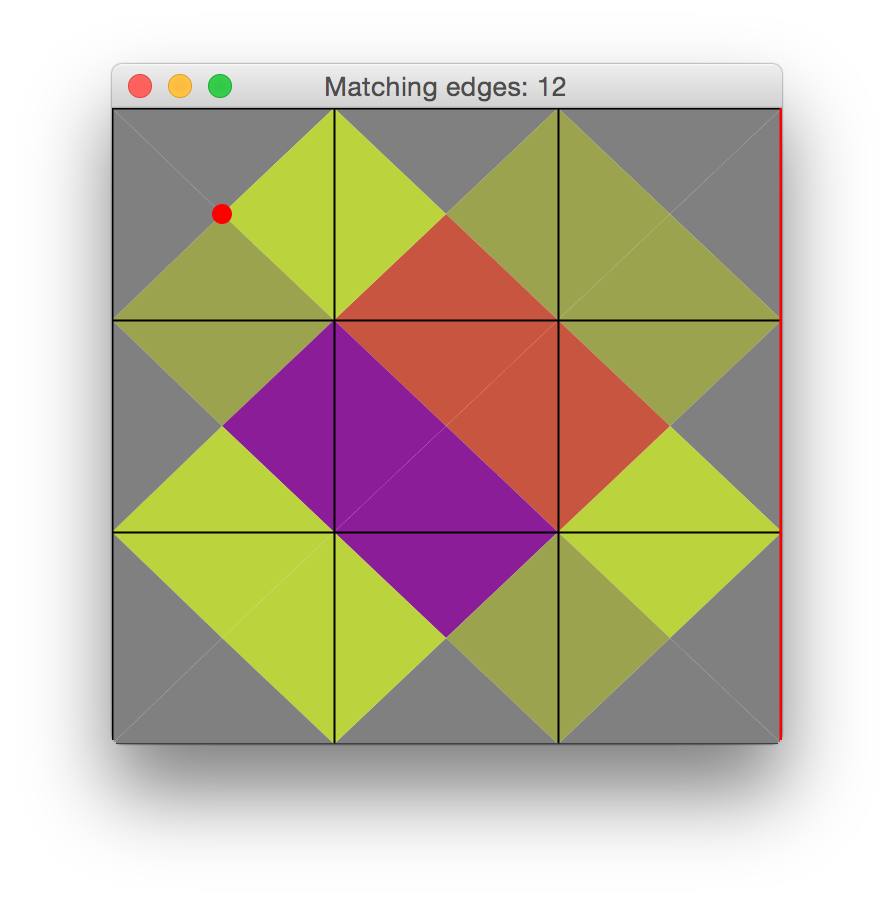
\includegraphics[scale=0.25]{img/sol_03x03_SA}
	\caption{Solution of the 3x3 board.}
	\end{figure}

	Per il resto delle istanze, si è visto la tecnica del simulated annealing non fornisce risultati paragonabili a quelli ottenuti usando la steepest descent.




	\subsection{Steepest Descent con mossa 5--modale}
	Come detto prima, si sono usati dei file interni per guidare il tester di easylocal++ durante la steepest descent. Questi file si trovano della cartella \emph{ourInput}. Nel seguito indicheremo i migliori risultati ottenuti tramite questa tecnica e la mossa 5--modale.

	\paragraph{03x03}
	\texttt{./Eternity2 --main::instance ../eternity2-data/pieces\_set\_2/pieces\_03x03.txt --main::seed 24 $<$ ../eternity2-data/ourInput/input\_03x03.txt $\mid$ tail -n 100}

	\begin{itemize}
		\item COST = 0
		\item TIME = 0.027 sec
	\end{itemize}
	\begin{figure}[H]
	\centering
	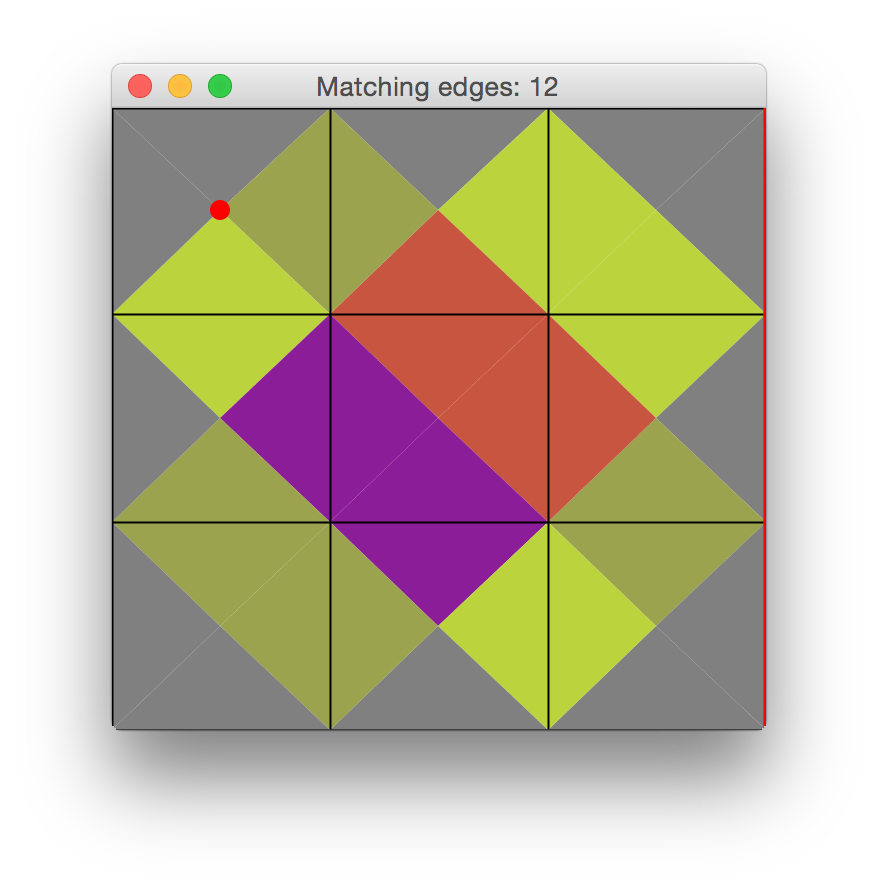
\includegraphics[scale=0.25]{img/sol_03x03}
	\caption{Solution of the 3x3 board.}
	\end{figure}



	\paragraph{04x04}
	\texttt{./Eternity2 --main::instance ../eternity2-data/pieces\_set\_2/pieces\_04x04.txt --main::seed 26 $<$ ../eternity2-data/ourInput/input\_04x04.txt $\mid$ tail -n 100}

	\begin{itemize}
		\item COST = 0
		\item TIME = 0.057 sec
	\end{itemize}
	\begin{figure}[H]
	\centering
	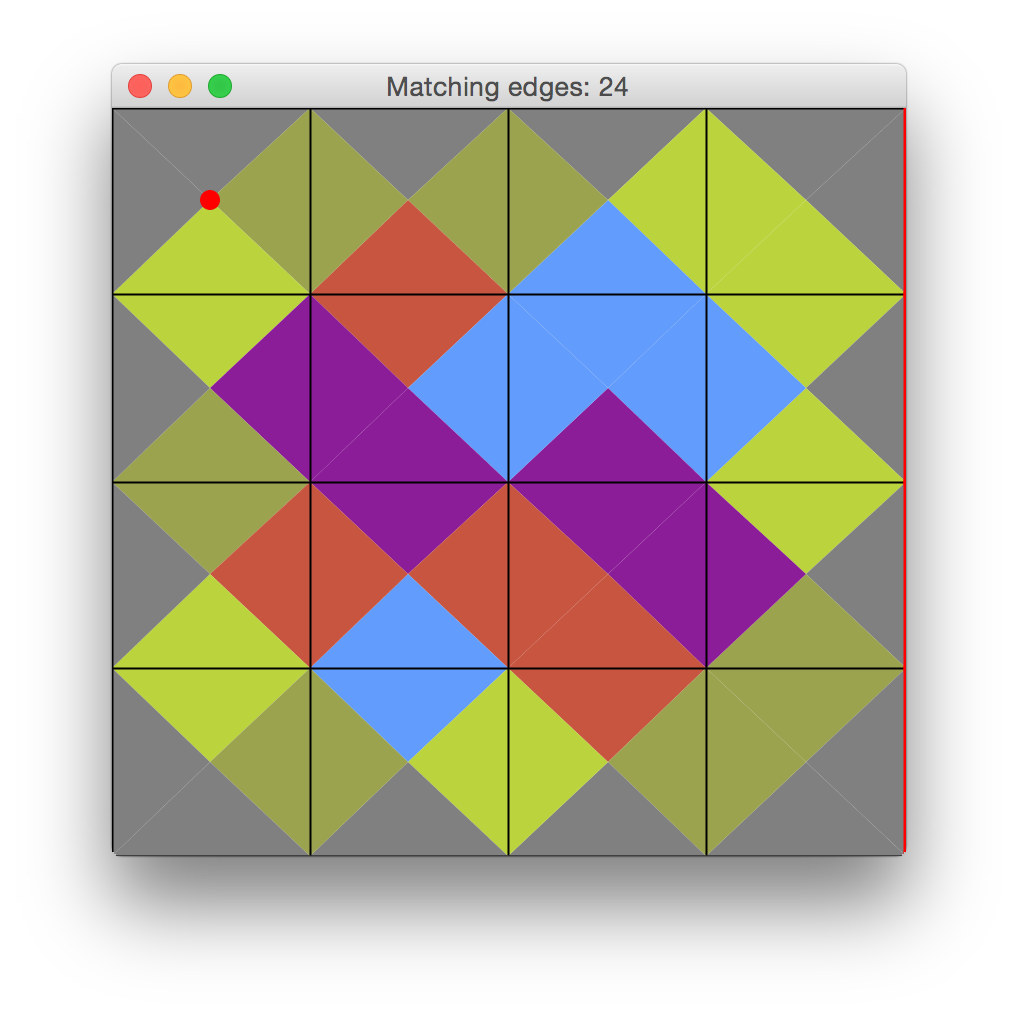
\includegraphics[scale=0.25]{img/sol_04x04}
	\caption{Solution of the 4x4 board.}
	\end{figure}



	\paragraph{05x05}
	\texttt{./Eternity2 --main::instance ../eternity2-data/pieces\_set\_2/pieces\_05x05.txt --main::seed 987 $<$ ../eternity2-data/ourInput/input\_05x05.txt $\mid$ tail -n 100}

	\begin{itemize}
		\item COST = 2000
		\item TIME = 1.734 sec
	\end{itemize}
	\begin{figure}[H]
	\centering
	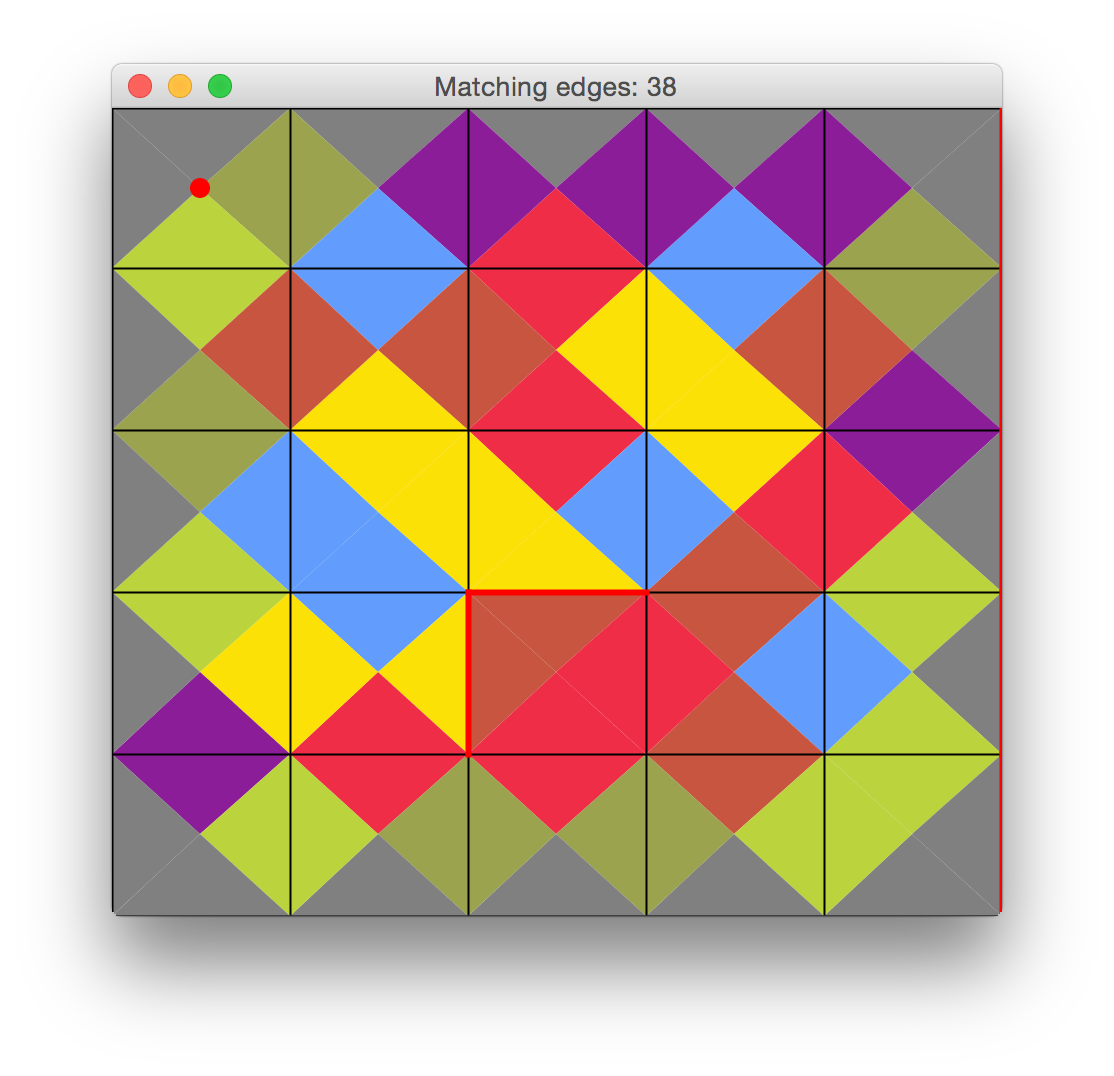
\includegraphics[scale=0.25]{img/sol_05x05}
	\caption{Solution of the 5x5 board.}
	\end{figure}



	\paragraph{06x06}
	\texttt{./Eternity2 --main::instance ../eternity2-data/pieces\_set\_2/pieces\_06x06.txt --main::seed 69 $<$ ../eternity2-data/ourInput/input\_06x06\_3.txt $\mid$ tail -n 150}

	\begin{itemize}
		\item COST = 3000
		\item TIME = 26.508 sec
	\end{itemize}
	\begin{figure}[H]
	\centering
	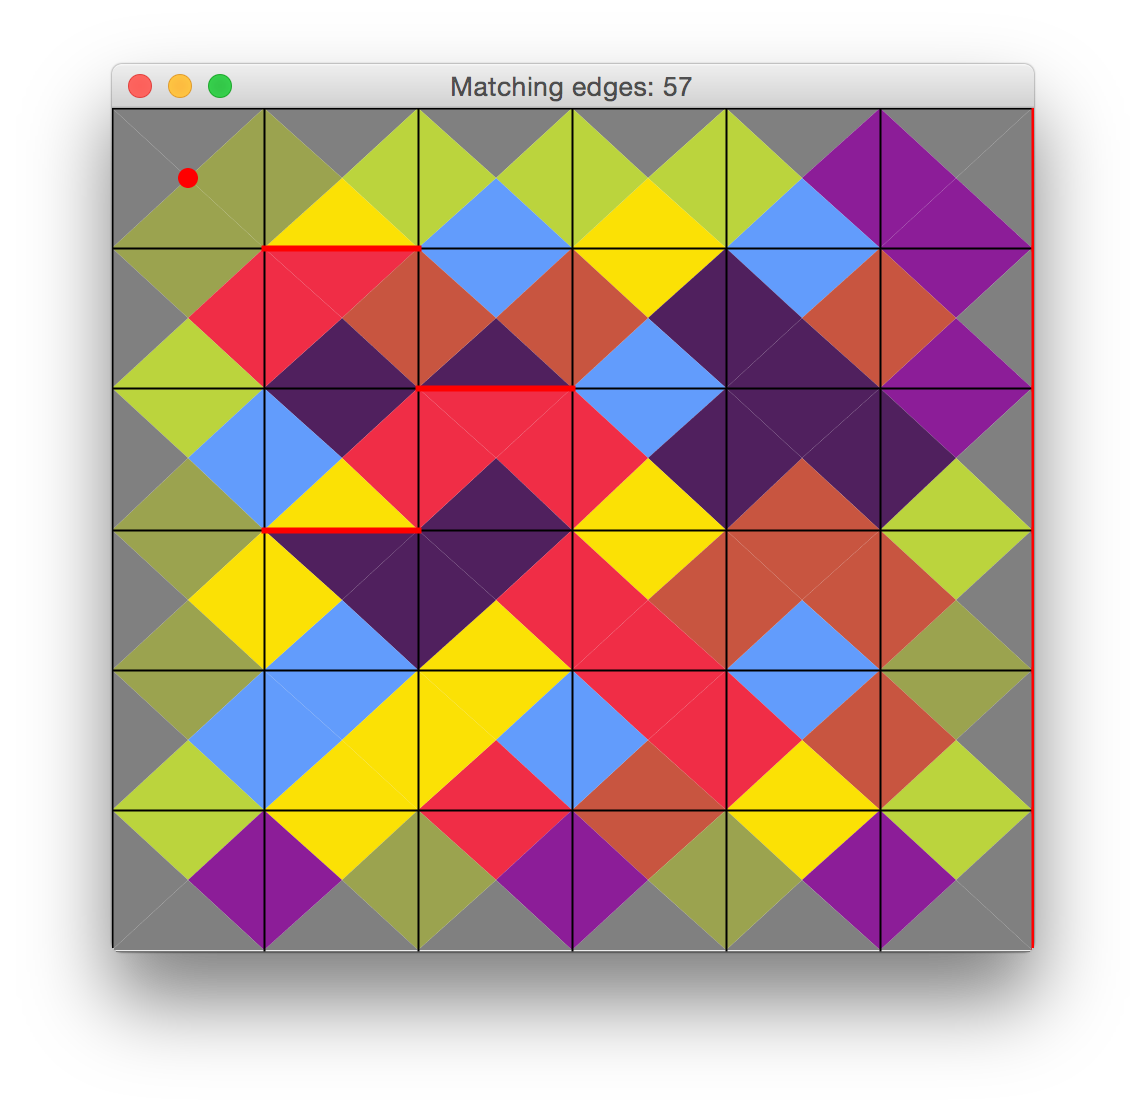
\includegraphics[scale=0.25]{img/sol_06x06}
	\caption{Solution of the 6x6 board.}
	\end{figure}



	\paragraph{07x07}
	\texttt{./Eternity2 --main::instance ../eternity2-data/pieces\_set\_2/pieces\_07x07.txt --main::seed 987 $<$ ../eternity2-data/ourInput/input\_07x07.txt $\mid$ tail -n 100}

	\begin{itemize}
		\item COST = 8000
		\item TIME = 5.552 sec
	\end{itemize}
	\begin{figure}[H]
	\centering
	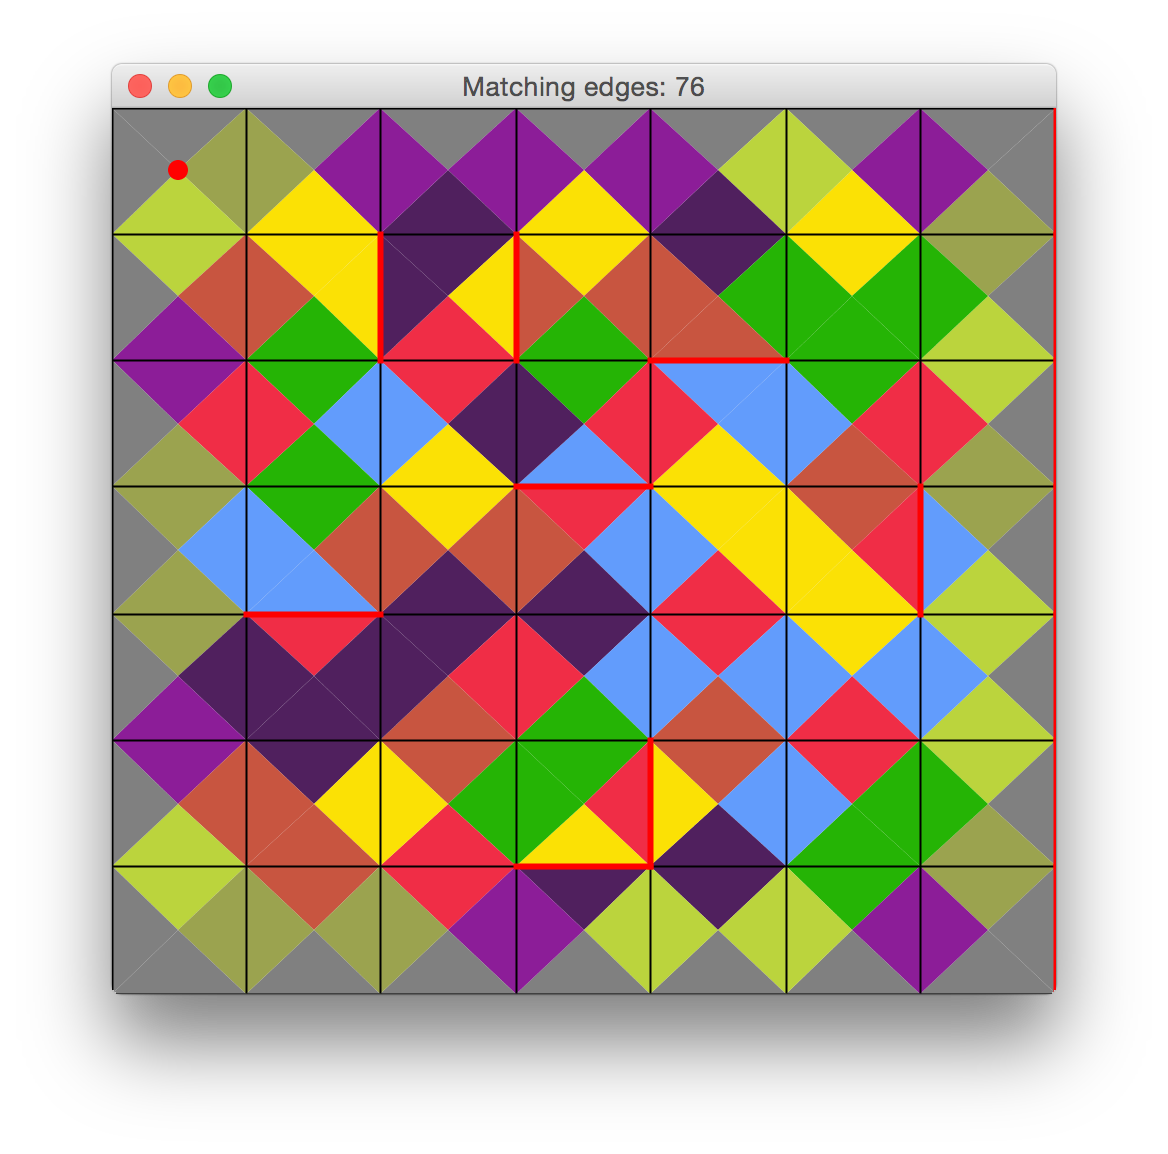
\includegraphics[scale=0.25]{img/sol_07x07}
	\caption{Solution of the 7x7 board.}
	\end{figure}



	\paragraph{08x08}
	

	\begin{itemize}
		\item COST = 15000
		\item TIME = 8.250 sec
	\end{itemize}
	\begin{figure}[H]
	\centering
	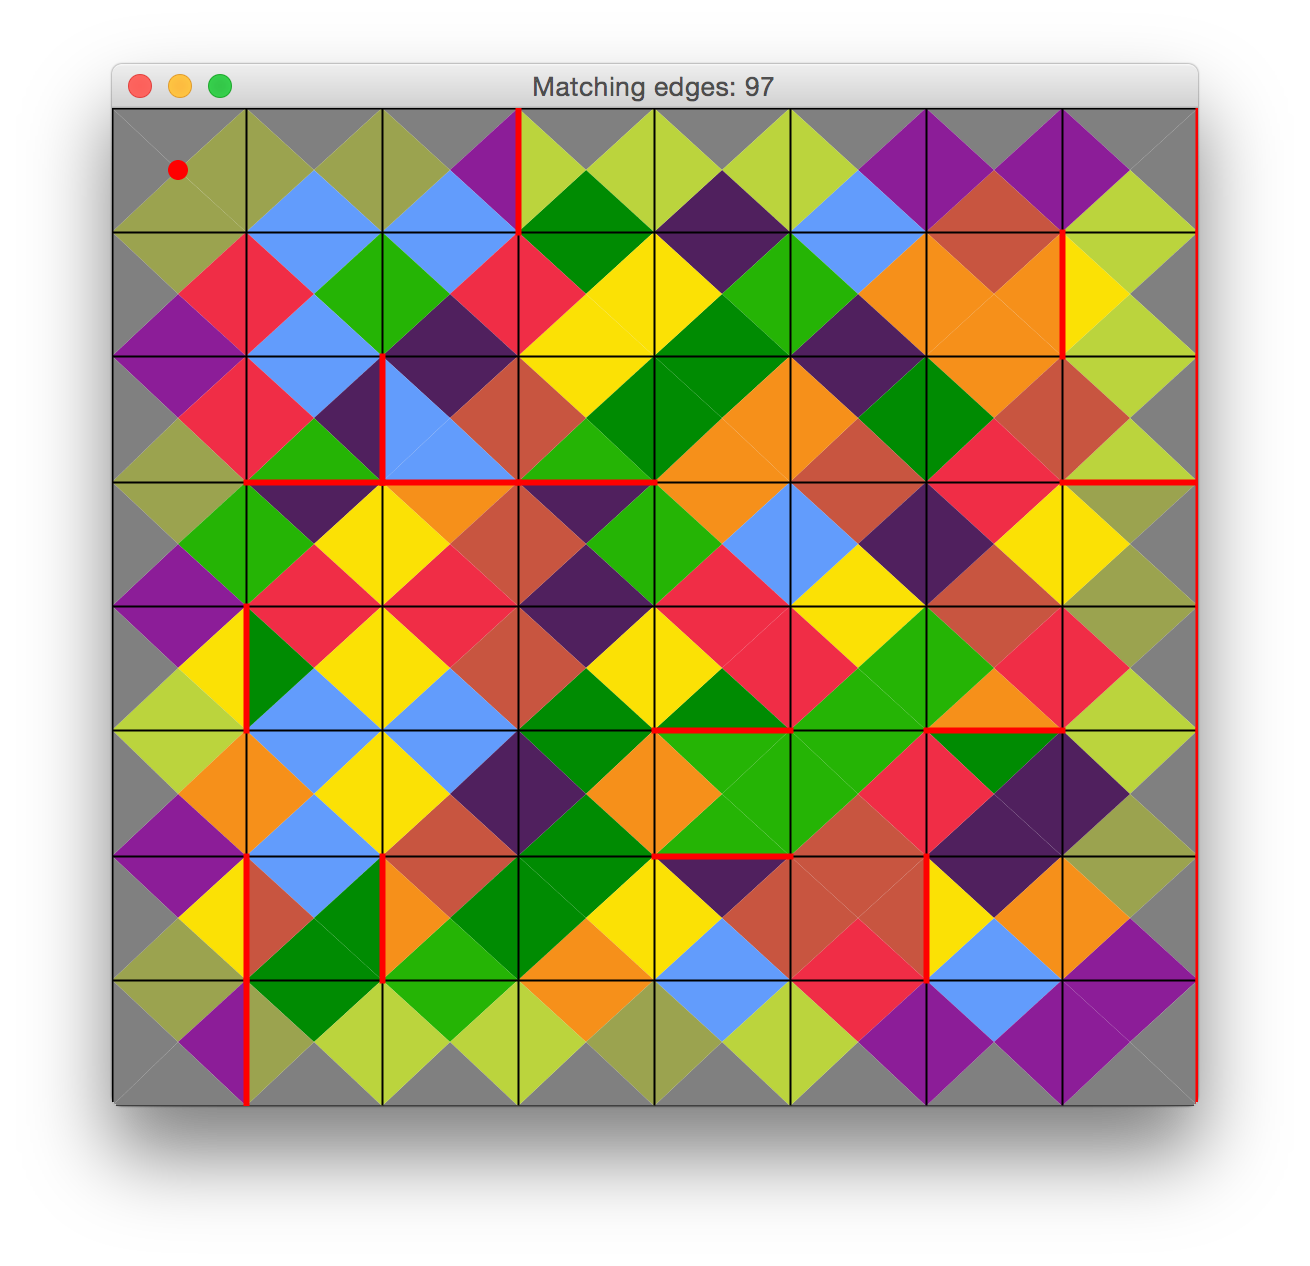
\includegraphics[scale=0.25]{img/sol_08x08}
	\caption{Solution of the 8x8 board.}
	\end{figure}



	\paragraph{09x09}
	\texttt{./Eternity2 --main::instance ../eternity2-data/pieces\_set\_2/pieces\_09x09.txt --main::seed 1 $<$ ../eternity2-data/ourInput/input\_09x09.txt $\mid$ tail -n 150 }

	\begin{itemize}
		\item COST = 19000
		\item TIME = 13.110 sec
	\end{itemize}
	\begin{figure}[H]
	\centering
	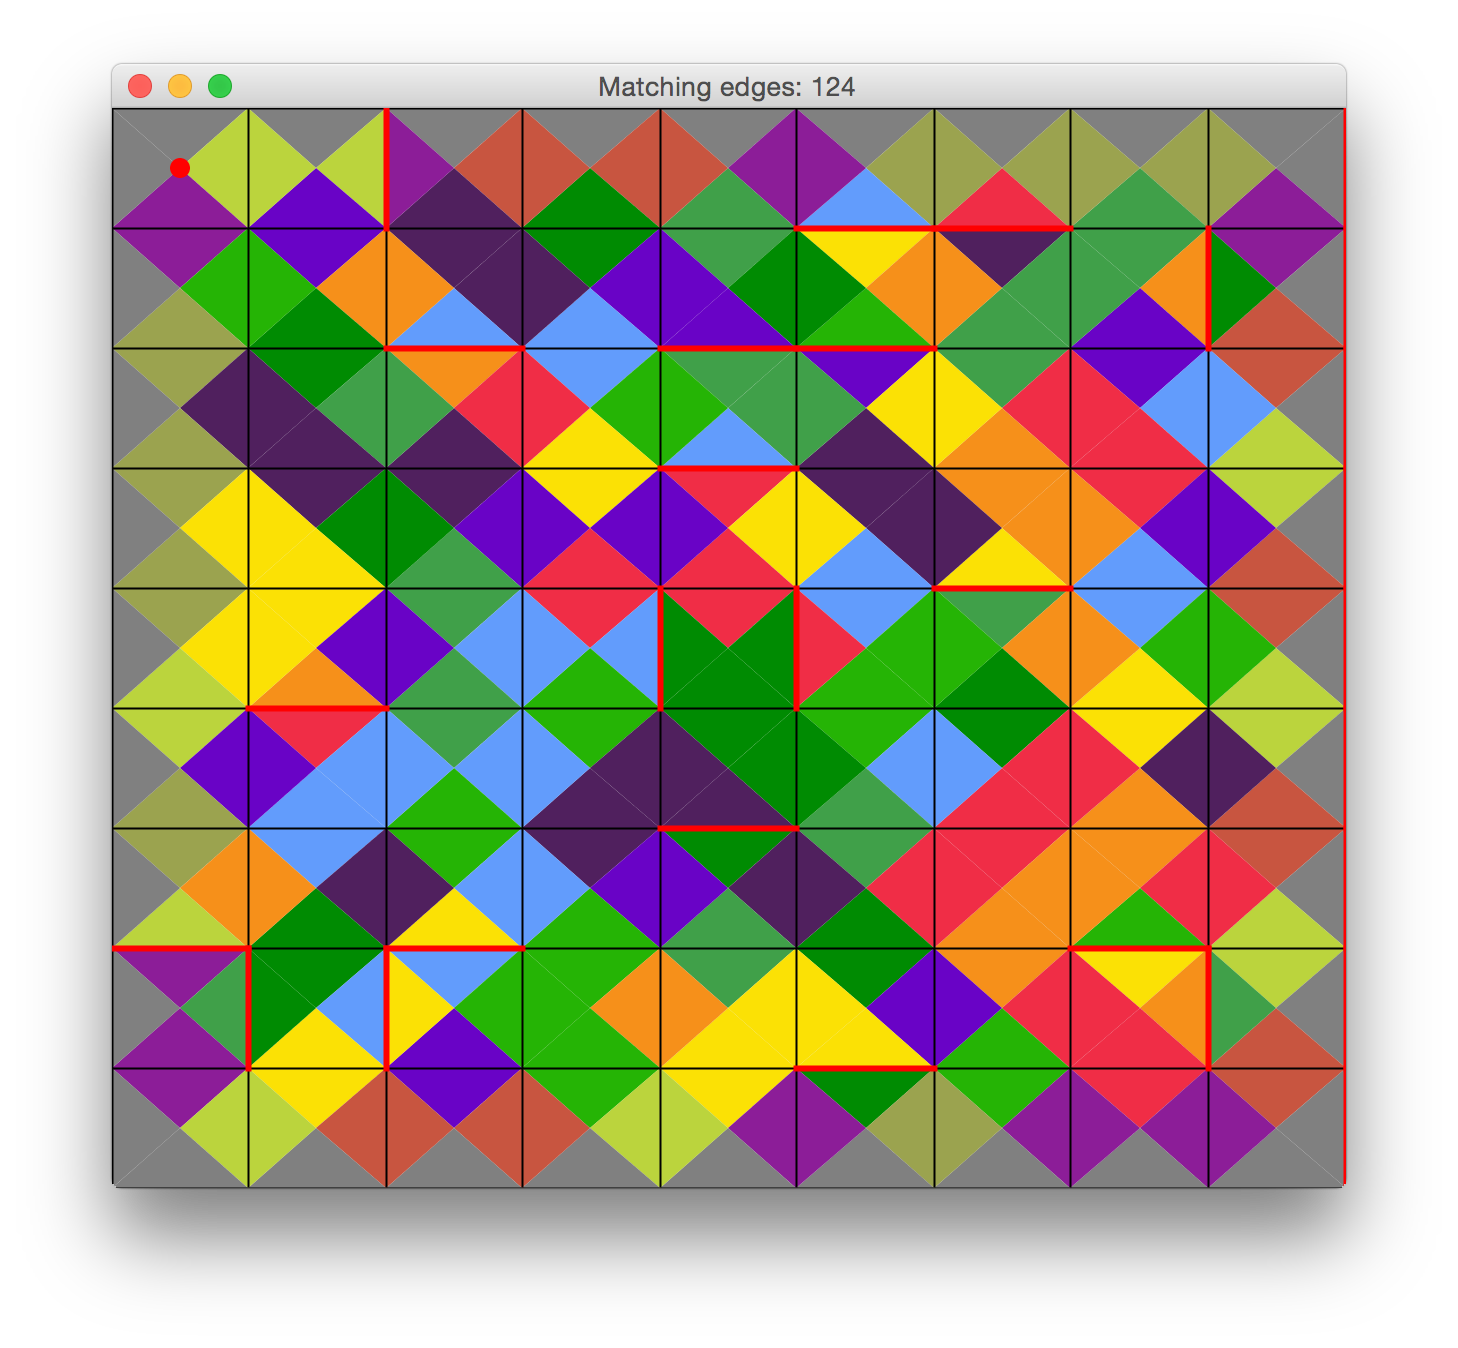
\includegraphics[scale=0.25]{img/sol_09x09}
	\caption{Solution of the 9x9 board.}
	\end{figure}



	\paragraph{10x10}
	\texttt{./Eternity2 --main::instance ../eternity2-data/pieces\_set\_2/pieces\_10x10.txt --main::seed 0 $<$ ../eternity2-data/ourInput/input\_10x10\_19.txt $\mid$ tail -n 150 }

	\begin{itemize}
		\item COST = 19000
		\item TIME = 23.397 sec
	\end{itemize}
	\begin{figure}[H]
	\centering
	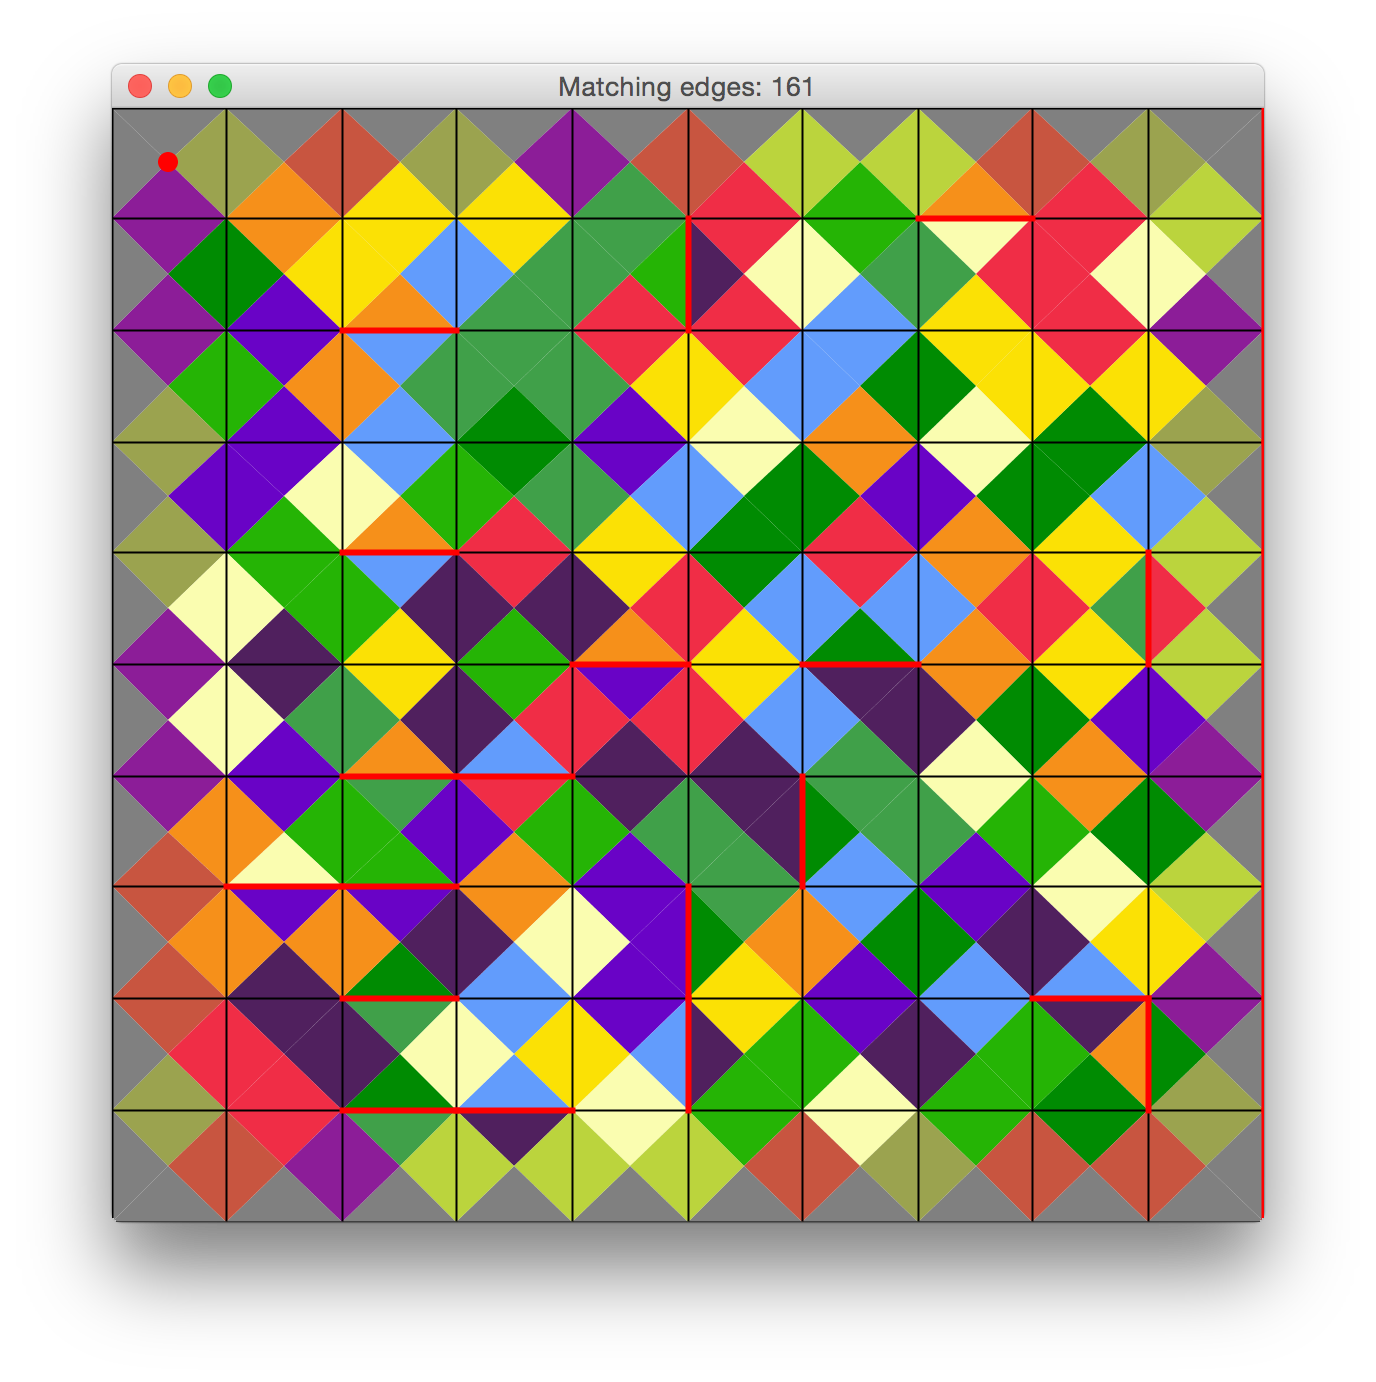
\includegraphics[scale=0.25]{img/sol_10x10}
	\caption{Solution of the 10x10 board.}
	\end{figure}



	\paragraph{11x11}
	\texttt{./Eternity2 --main::instance ../eternity2-data/pieces\_set\_2/pieces\_11x11.txt --main::seed 351 $<$ ../eternity2-data/ourInput/input\_11x11\_24.txt $\mid$ tail -n 150}

	\begin{itemize}
		\item COST = 24000
		\item TIME = 7 m 30 sec
	\end{itemize}
	\begin{figure}[H]
	\centering
	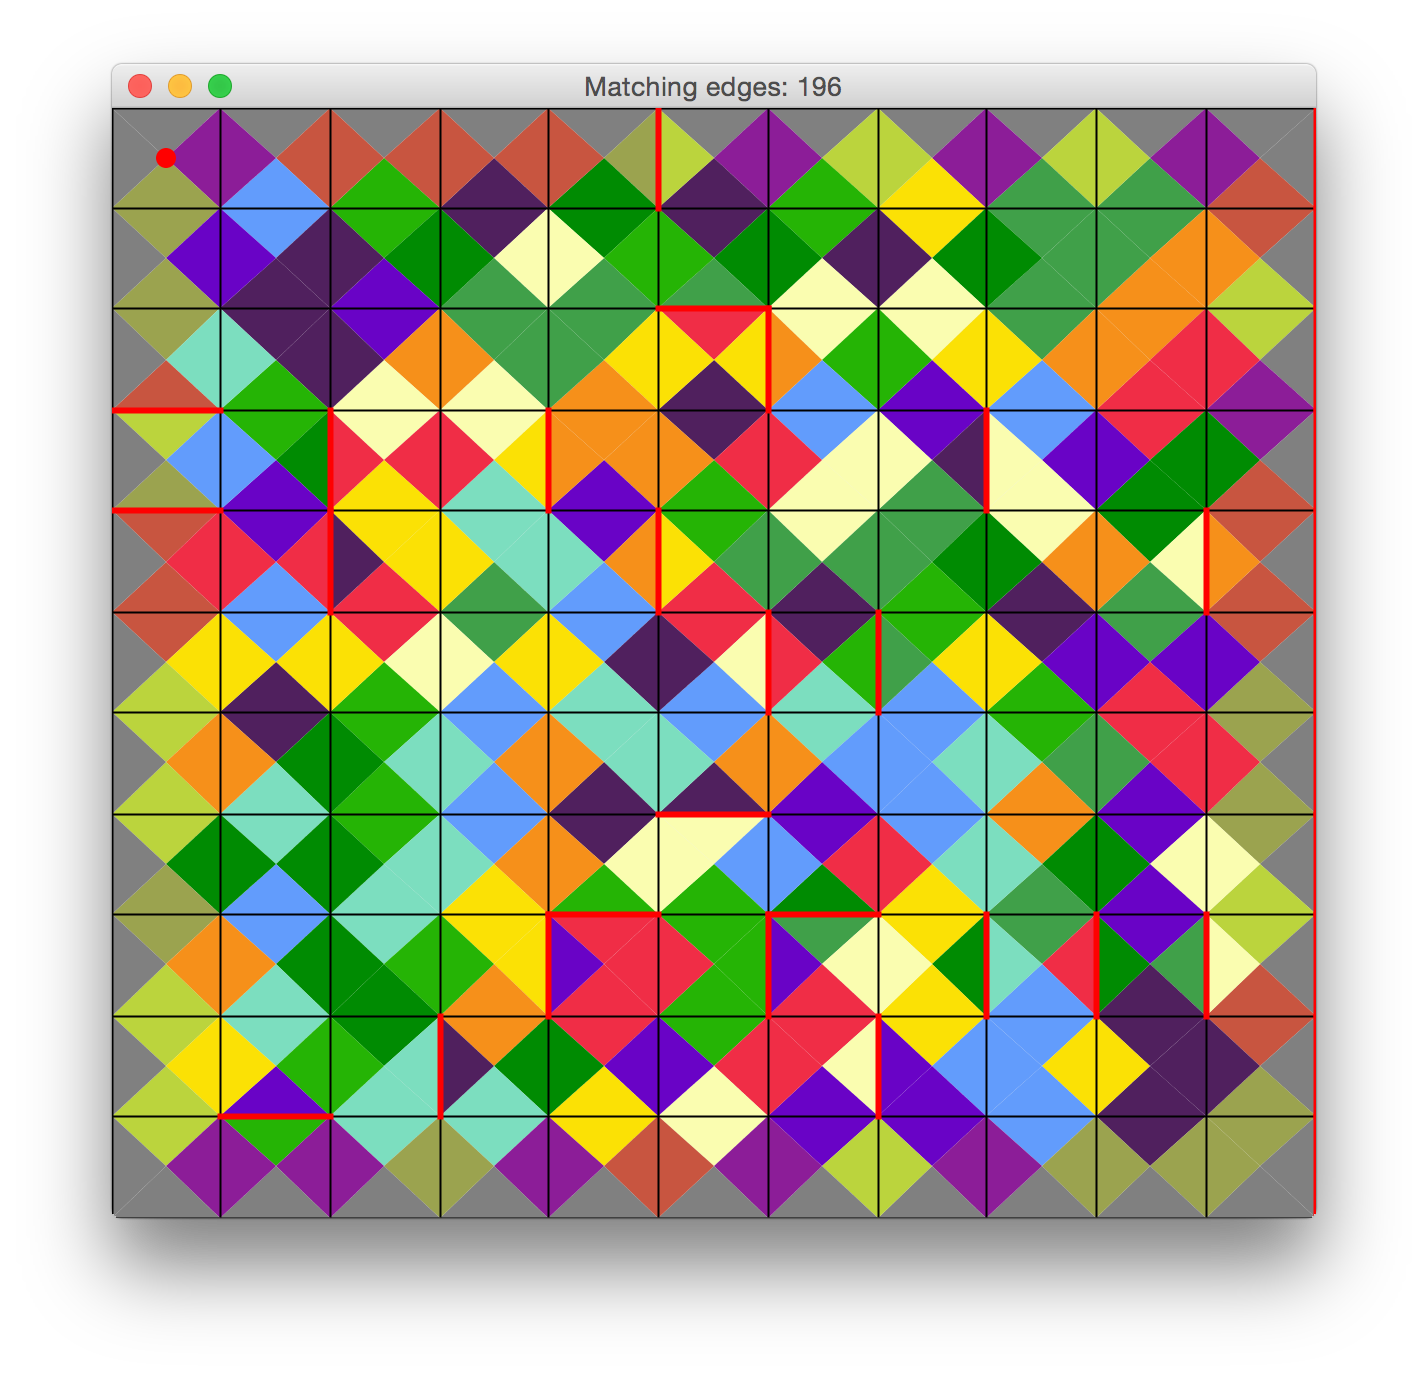
\includegraphics[scale=0.25]{img/sol_11x11}
	\caption{Solution of the 11x11 board.}
	\end{figure}



	\paragraph{12x12}
	\texttt{./Eternity2 --main::instance ../eternity2-data/pieces\_set\_2/pieces\_12x12.txt --main::seed 479 $<$ ../eternity2-data/ourInput/input\_12x12\_32.txt $\mid$ tail -n 150}

	\begin{itemize}
		\item COST = 32000
		\item TIME = 13 m 42 sec
	\end{itemize}
	\begin{figure}[H]
	\centering
	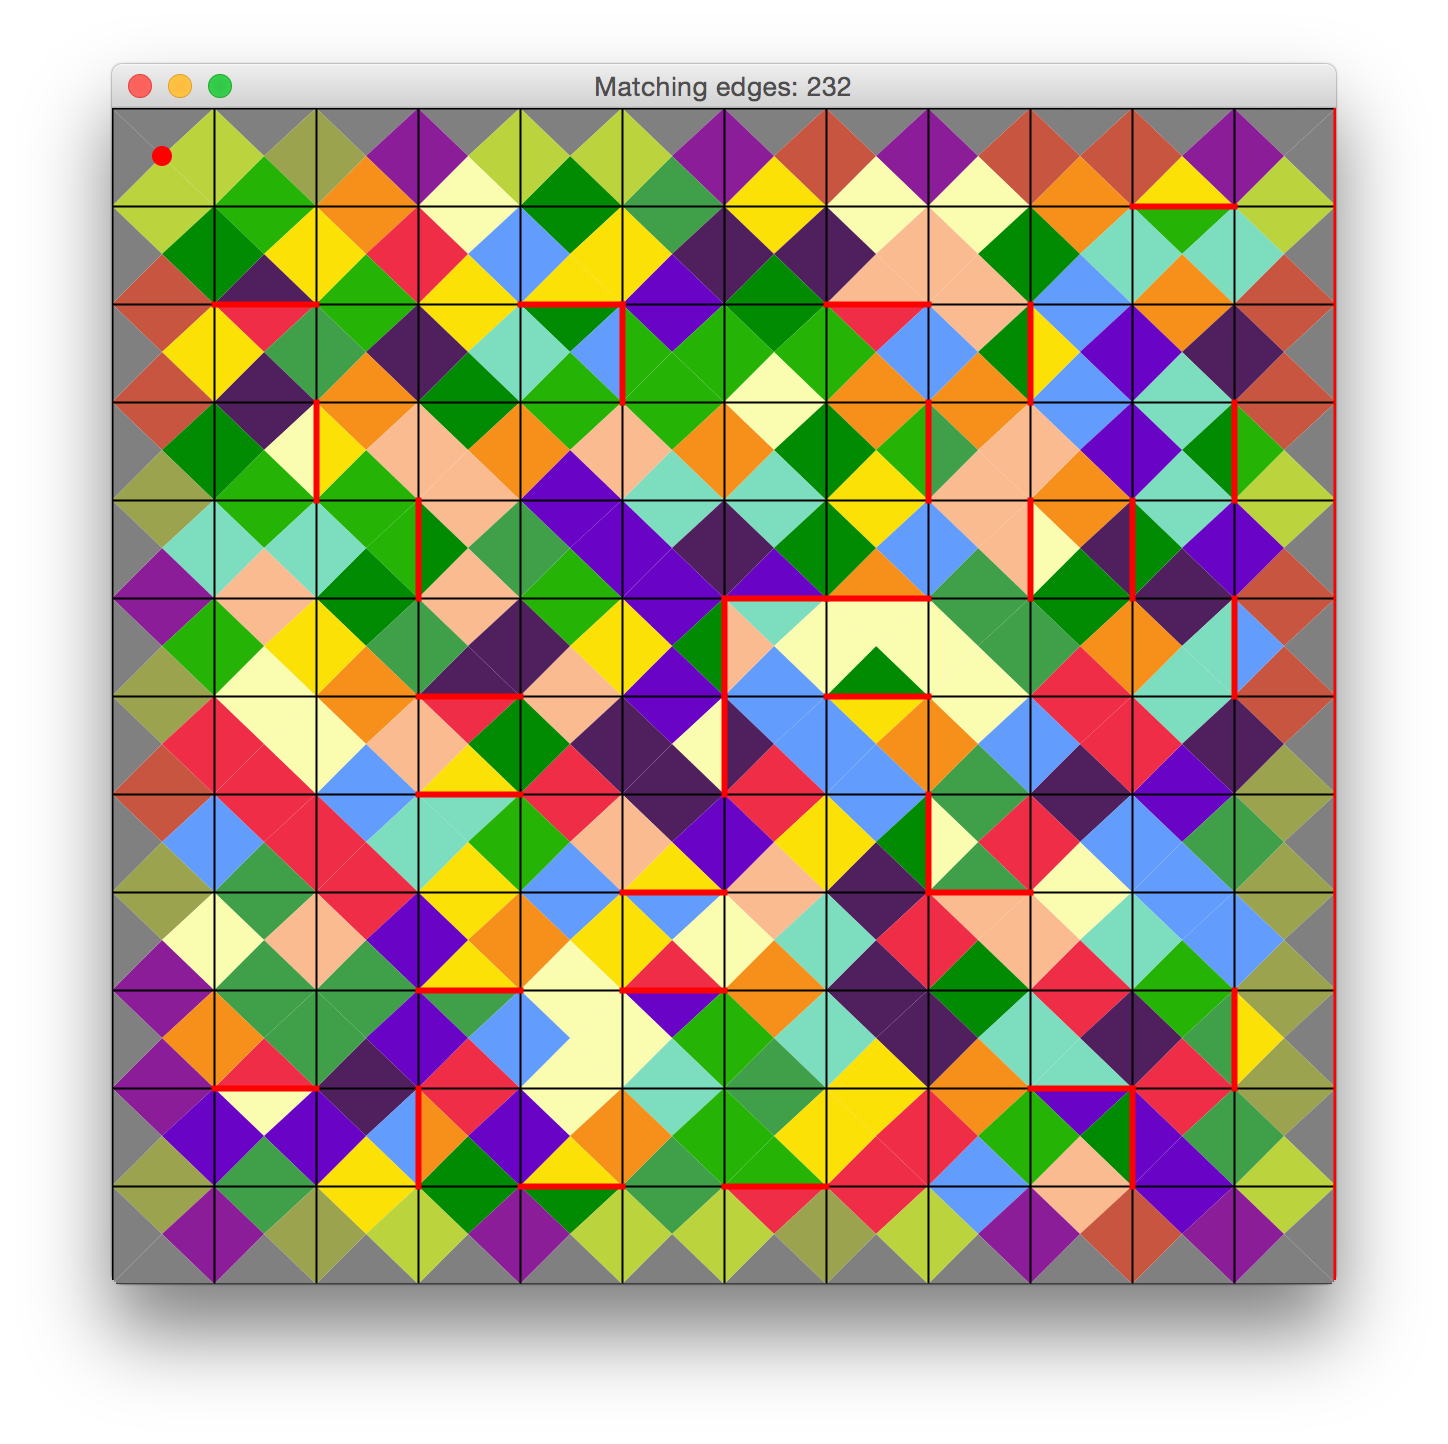
\includegraphics[scale=0.25]{img/sol_12x12}
	\caption{Solution of the 12x12 board.}
	\end{figure}



	\paragraph{13x13}
	\texttt{./Eternity2 --main::instance ../eternity2-data/pieces\_set\_2/pieces\_13x13.txt --main::seed 22 $<$ ../eternity2-data/ourInput/input\_13x13\_41.txt $\mid$ tail -n 150}

	\begin{itemize}
		\item COST = 41000
		\item TIME = 10 min 4 sec
	\end{itemize}
	\begin{figure}[H]
	\centering
	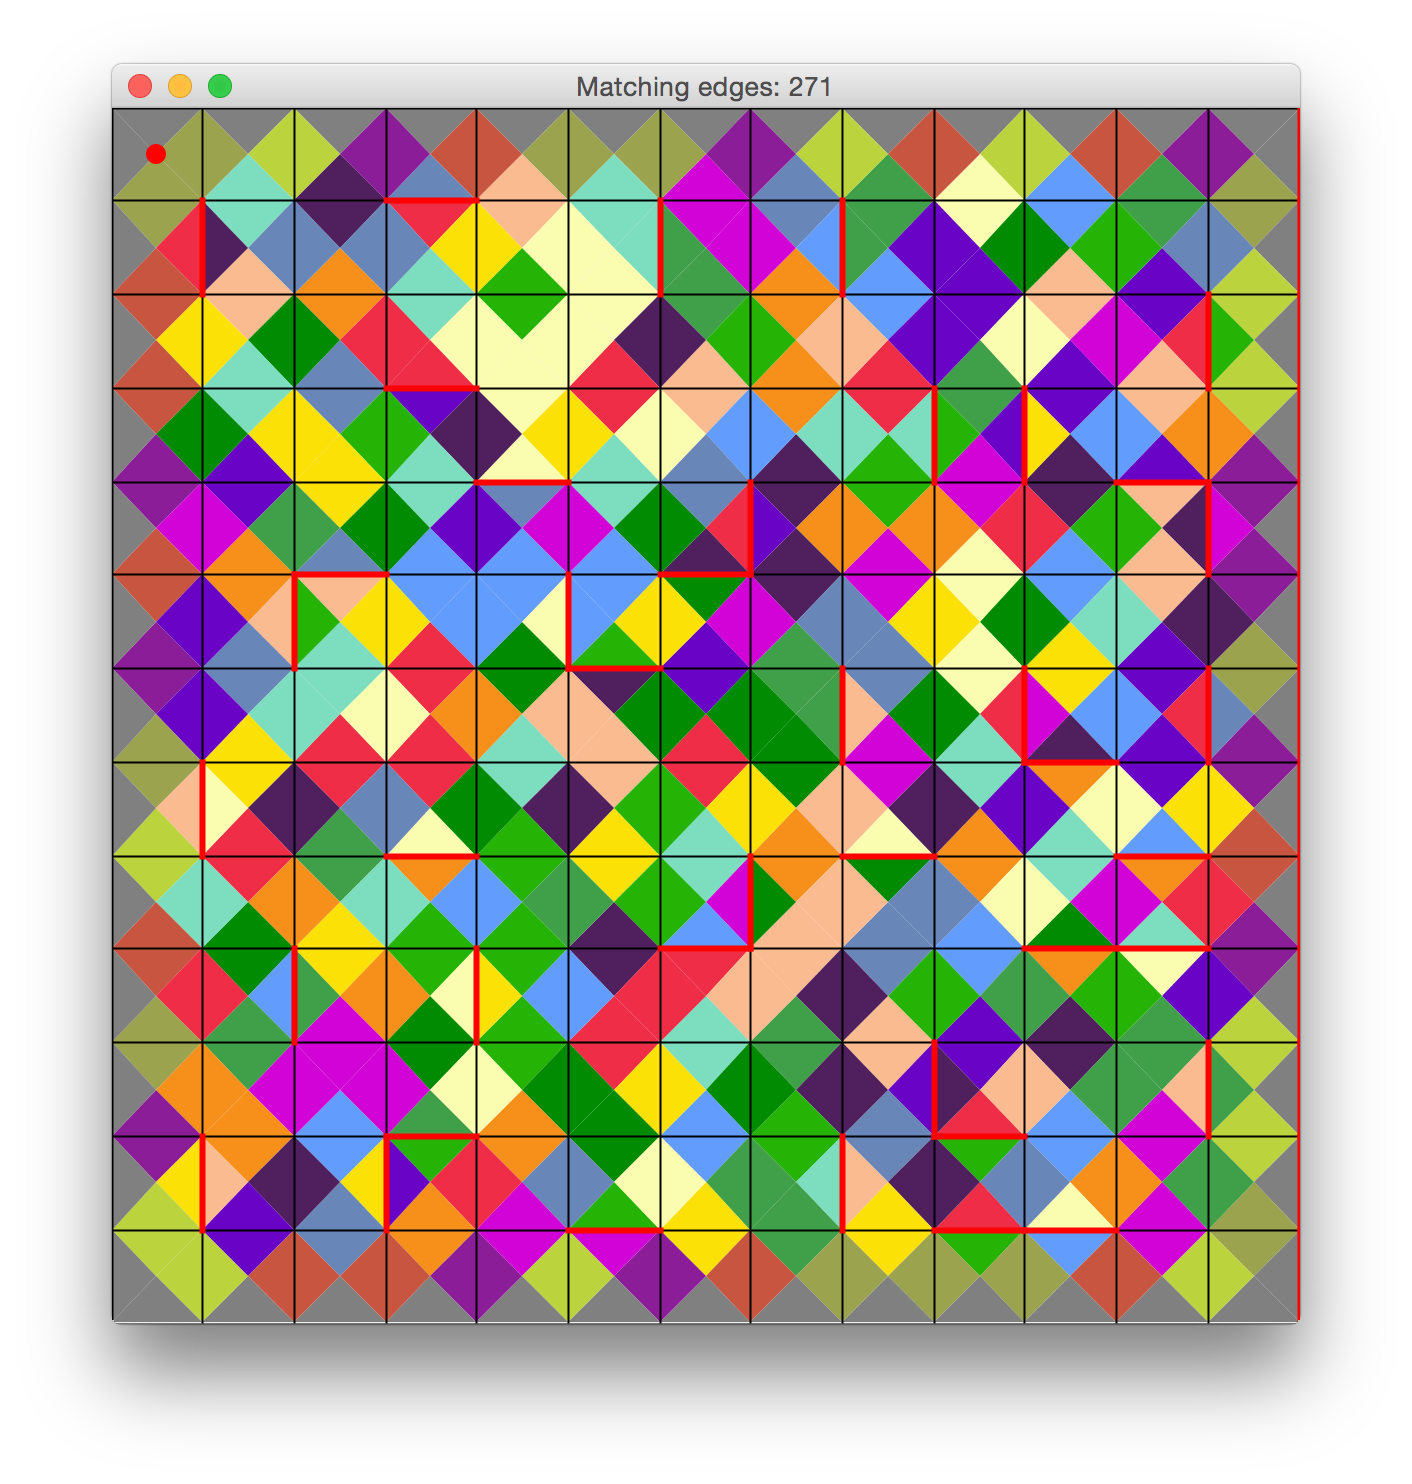
\includegraphics[scale=0.25]{img/sol_13x13}
	\caption{Solution of the 13x13 board.}
	\end{figure}



	\paragraph{Eternity 2 originale}
	\texttt{./Eternity2 --main::instance ../eternity2-data/pieces\_set\_2/e2pieces.txt --main::seed 987 $<$ ../eternity2-data/ourInput/input\_e2.txt $\mid$ tail -n 100}

	\begin{itemize}
		\item COST = 62000
		\item TIME = 3 m 40 sec
	\end{itemize}
	\begin{figure}[H]
	\centering
	\includegraphics[scale=0.5]{img/sol_e2}
	\caption{Solution of Eternity 2.}
	\end{figure}














% section test (end)